% displayname : Puits de potentiel
\documentclass[12pt,fancy]{cours}
\Chapit{6}{8}
\begin{document}
\maketitre[***]{
  Nous appliquons les principes de la mécanique quantique ondulatoire à deux problèmes simples. D'abord, l'étude de particules confinées dans un puits de potentiel, que l'on modélise par un puits infini puis un puits fini. Puis la transmission de particules à travers une barrière de potentiel, phénomène que l'on appelle l'effet tunnel. Cet effet est à la base de la microscopie à effet tunnel et du mécanisme de désintégration alpha.
}
{
\item Cours de Physique quantique - 0
\item Document de cours Physique quantique - 1
\item TD Physique quantique
}

%%%%%%%%%%%%%%%%%%%%%%%%%%%%%%%%%%%%%%%%%%%%%%%%%%%%%%%%
\section{Le puits de potentiel infini}
\subsection{Position du problème}

Considérons une particule piégée dans un puits de potentiel de profondeur infinie à une dimension (Fig.~\ref{fig:puits_infini}) tel que
\begin{equation}
V(x) =
\begin{cases}
0 & \mbox{si } 0<x<a, \\
+\infty & \mbox{sinon}.
\end{cases}
\end{equation}
Ce type de potentiel décrit en première approximation toute particule quantique confinée, par exemple les nucléons dans le noyau atomique, les électrons autour du noyau atomique, etc.
\begin{figure}[H]
  \centering
  
\includegraphics[width=0.5\textwidth]{infinite_trap.pdf}
  \caption{Puits de potentiel infini (la zone colorée correspond aux régions interdites, de potentiel infini).}
  \label{fig:puits_infini}
\end{figure}

%En mécanique classique, une particule de masse $m$ dans ce potentiel a son énergie totale $E$ conservée, qui est la somme de son énergie cinétique et de son énergie potentielle. L'énergie étant finie, cela interdit à la particule de se trouver en dehors de l'intervalle $[0,L]$. Dans cet intervalle, la probabilité de présence de la particule moyennée sur les conditions initiales est une distribution rectangulaire indépendante du temps égale à $\rho(x)=1/L$. Par ailleurs, il n'y a aucune contrainte sur l'énergie. Autrement dit, elle peut prendre n'importe quelle valeur $E>0$ (elle doit être supérieure au potentiel, qui est pris nul par convention).

\subsection{Modes propres et quantification}

\parag{Modes propres}
On recherche les états stationnaires dans ce puits infini. Dans le domaine $x \in [0,L]$, $V(x)=0$, et donc l'équation de Schrödinger indépendante du temps se simplifie en
\begin{equation}
-\frac{\hbar^2}{2m}\frac{\d^2\varphi}{\d x^2}=E\varphi
\quad\Rightarrow\quad\ddm{\varphi}{x}{2}+\frac{2mE}{\hbar^2}\varphi=0.
\label{eqn:schro_puits_infini}
\end{equation}
On reconnaît une équation différentielle du second ordre à coefficients constants: la forme de la solution dépend du signe de $E$.

\begin{liste}
  \item \udl{$E<0$} : la solution est exponentielle,
 \begin{equation}
 \varphi(x)=A\,\e^{k x}+B\,\e^{-k x}\quad\text{avec}\quad k=\sqrt{\frac{-2mE}{\hbar^2}},
 \end{equation}
 et $A$, $B$ deux constantes déterminées par les conditions aux limites. Ici, on exploite la continuité de la fonction d'onde en $x=0$ et $x=a$ : la probabilité de présence de la particule est nulle en dehors de $[0,a]$ car le potentiel est infini, donc
 \begin{equation}
 \varphi(0)=\varphi(a)=0.
 \label{eqn:cls_puits_inf}
 \end{equation}

 On aboutit alors au système suivant vérifié par les constantes d'intégration :
 \begin{equation}
 \begin{cases}
 A+B=0,\\
 A\,\e^{ka}+ B\,\e^{-ka}=0.
 \end{cases}
 \end{equation}
 La seule solution est $A=B=0$. Il n'existe donc pas de solution non triviale avec $E<0$. %C'est également ce que donne un raisonnement purement classique.
\item \udl{$E>0$} : on reconnaît un oscillateur harmonique, dont la solution est sinusoïdale,
\begin{equation}
\varphi(x)=A\cos(kx)+B\sin(kx)\quad\text{avec}\quad k=\sqrt{\frac{2mE}{\hbar^2}}
\end{equation}
le vecteur d'onde.
Les conditions aux limites donnent
\begin{equation}
  \begin{cases}
  \varphi(0)=0,\\
  \varphi(a)=0.
  \end{cases}
 \Rar    \begin{cases}
   A=0,\\
   B\sin(ka)=0.
   \end{cases}
\end{equation}
On peut avoir une fonction d'onde non nulle si $\sin(ka)=0$ : il existe $n$ entier tel que
\begin{equation}
k_n=\frac{n\pi}{a}.
\end{equation}
Une telle solution est appelée \imp{mode propre}.
L'énergie d'un mode propre vaut
\begin{equation}
E_n=\frac{\hbar^2 k_n^2}{2m}=n^2\frac{\hbar^2\pi^2}{2ma^2}.
\end{equation}
Ainsi, le vecteur d'onde et l'énergie d'un mode propre sont \imp{quantifiées}.
%
% où $E_1 = \frac{\hbar^2\pi^2}{2mL^2}$ est l'énergie du fondamental, appelée énergie de point zéro.
% Cette quantification \important{est une conséquence du confinement de la particule}, et résulte de la description ondulatoire de la matière. On retrouve un phénomène similaire à la quantification des modes propres stationnaires d'une corde fixée à ses deux extrémités.
\end{liste}

\begin{remarque}
On ne peut pas utiliser de condition sur la dérivée première de $\varphi(x)$ car le potentiel présente une discontinuité infinie. Mais ceci n'est pas nécessaire car il y a deux conditions aux limites pour deux coefficients à déterminer.
\end{remarque}

\begin{prop}[Modes propres]\label{prop:}
Les états stationnaires d'une particule \imp{confinée} dans un puits de potentiel infini sont appelés \imp{modes propres}. Le vecteur d'onde et l'énergie d'un mode propre sont \imp{quantifiées} suivant
\begin{equation*}
  k_n=\frac{n\pi}{a}, \qquad E_n=n^2E_1, 
\end{equation*}
avec $n\geq1$ entier et $E_1=\frac{\hbar^2\pi^2}{2m a^2}$ l'énergie de point zéro.
\end{prop}

\parag{Énergie de point zéro} Le mode propre fondamental, pour $n=1$, est le mode d'énergie la plus faible. Cependant, cette énergie est non nulle, et vaut
\begin{equation}
  E_1=\frac{\hbar^2\pi^2}{2m a^2}.
\end{equation}
Cette énergie minimale est appelée énergie de point zéro. 
% L'énergie de l'harmonique $n$ s'écrit alors $E_n = n^2 E_1$.

Contrairement au cas classique, dans l'état de plus basse énergie, la particule quantique n'est pas au repos: c'est une conséquence du confinement de la particule et du principe d'indétermination de Heisenberg. En effet, l'indétermination sur la position de la particule est de l'ordre de $\Delta x \sim a$. D'après le principe d'indétermination de Heisenberg, l'indétermination sur l'impulsion vaut $\Delta p \geq \frac{\hbar}{2a}$. Comme la valeur moyenne de l'impulsion est nulle, $\Delta p$ représente aussi l'ordre de grandeur de l'impulsion elle-même. On en déduit que l'énergie de la particule vérifie
\begin{equation}
E\sim\frac{\Delta p^2}{2m}\geq \frac{\hbar^2}{8ma^2}\sim E_1.
\end{equation}
On retrouve alors l'énergie de point zéro $E_1$ comme énergie minimale.

% \begin{remarquetech}
% On retiendra que lorsqu'une particule est confinée dans une région de taille caractéristique $L$, elle présente une énergie cinétique minimale due au confinement qui vaut
% \begin{equation}
% E_{\mathrm{c},\mathrm{min}}\simeq\frac{\hbar^2}{mL^2}.
% \label{eqn:energie_confinement}
% \end{equation}
% Cette énergie est d'autant plus importante que le puits est étroit ($a$ petit).
% \end{remarquetech}



\subsection{Expression de la fonction d'onde}


Les fonctions d'onde spatiales associées aux états propres sont donc de la forme $\varphi_n(x)=A_n\sin(n\pi x/a)$. Le facteur $A_n$ s'obtient en normalisant la fonction d'onde
\begin{equation}
1 = \int_0^a\left\vert\varphi_n(x)\right\vert^2\d x= A_n^2 \int_0^a\sin^2\left(\frac{n\pi x}{a}\right)\d x=\left\vert A_n\right\vert^2\frac{a}{2} \Rar A_n=\sqrt{\frac{2}{a}},
\end{equation}
à une phase globale près.
On en déduit
\begin{equation}
\varphi_n(x)=\sqrt{\frac{2}{a}}\sin\left(\frac{n\pi x}{a}\right).
\end{equation}
%
% Dans le cas quantique il existe un nouveau phénomène: en plus du vecteur d'onde, l'énergie de l'onde (ou de la particule selon l'interprétation) est aussi quantifiée et vaut $\forall n\in\mathbb{N}^{\star}$
% \begin{equation}
% E_n=\frac{(\hbar k_n)^2}{2m}=n^2\frac{\hbar^2\pi^2}{2mL^2}\propto n^2.
% \label{eqn:energie_puits_infini}
% \end{equation}
% Cette expression provient du lien entre l'énergie de la particule et le vecteur d'onde, obtenu par la relation de dispersion.
L'expression complète de la fonction d'onde du mode propre $n$ s'obtient par $\psi_n(x,t)=\varphi_n(x)\,\e^{-iE_nt/\hbar}$.

\begin{figure}[H]
  \centering
  
\includegraphics[width=0.7\textwidth]{modes_propres.jpg}
  \caption{Densité de probabilité des premiers modes propres pour un puits infini. On notera l'analogie forte avec les modes propres d'une corde vibrante attachée à ses deux extrémités.}
\end{figure}
\begin{theorem}[Fonction d'onde des modes propres]\label{form:}
  Le mode propre d'ordre $n$, d'énergie $E_n$, a pour fonction d'onde
  \begin{equation*}
  \psi_n(x,t)=\sqrt{\frac{2}{a}}\sin\left(\frac{n\pi x}{a}\right)\,\e^{-iE_n t/\hbar}.
  \label{eqn:psi_puits_infini}
\end{equation*}
\end{theorem}

La distribution de probabilité de présence (indépendante du temps pour les modes propres qui sont des états stationnaires) est non uniforme et s'écrit
\begin{equation}
\rho_n(x)=\frac{2}{a}\sin^2\left(\frac{n\pi x}{a}\right).
\end{equation}
En particulier, elle s'annule aux bords de la zone de confinement, mais peut également présenter des n\oe{}uds et des ventres à des positions intermédiaires, comme le montre la Fig.~\ref{fig:puits_infini}.
 % Cela signifie qu'il existe des régions où la particule ne peut pas se trouver si elle possède une certaine énergie.

%
% \subsection{Énergie de point zéro}
% On vient de montrer que les énergies de la particule quantique dans le puits infini étaient quantifiées. En particulier, il existe un \important{fondamental}, c'est-à-dire un niveau de plus faible énergie. Ce fondamental a une énergie non nulle $E_1=\frac{\hbar^2\pi^2}{2m L^2}$. Il s'agit là d'un effet purement quantique. Cette énergie minimale d'une particule s'appelle \important{énergie de point zéro}. Nous allons montrer que contrairement au cas classique, dans l'état de plus basse énergie la particule quantique n'est jamais au repos: c'est une conséquence du confinement de la particule et du principe d'indétermination de Heisenberg.
% %
\section{Le puits de potentiel fini}
\subsection{Position du problème}


Nous traitons maintenant un problème un peu plus réaliste, qui est celui du puits fini schématisé en Fig.~\ref{fig:puits_fini} et caractérisé par le potentiel
\begin{equation}
V(x)=\begin{cases}
V_0 & \mbox{si } x<-\frac{a}{2} \text{ (région I)},\\
0 & \mbox{si } -\frac{a}{2}<x<\frac{a}{2} \text{ (région II)},\\
V_0 & \mbox{si } x>\frac{a}{2} \text{ (région III)},
\end{cases}
\end{equation}
avec $V_0>0$. Le puits infini correspond à la limite $V_0\to+\infty$.

\begin{figure}[H]
  \centering
  
\includegraphics[width=0.55\textwidth]{finite_trap.pdf}
  \caption{Représentation du puits de potentiel fini.}
  \label{fig:puits_fini}
\end{figure}

Le cas où $E<0$ se traite de la même façon que pour le puits infini: on montre qu'il n'existe pas de solution stationnaire. Il reste deux cas. Celui où $E>V_0$ correspond à un état où l'énergie de la particule n'est pas quantifiée : la particule n'est donc pas confinée à l'intérieur du puits. Dans toute la suite on se focalise sur le dernier cas d'un \imp{état lié}, pour lequel
\begin{equation}
  0<E<V_0,
\end{equation}
et on recherche des solutions stationnaires.

\subsection{Expression générale de la fonction d'onde}
\noindent L'équation de Schrödinger indépendante du temps s'écrit
\begin{equation}
\begin{cases}
\frac{\d^2\varphi}{\d x^2}+\frac{2m\left(E-V_0\right)}{\hbar^2}\varphi=0\quad\text{(régions I et III)},\\[2mm]
\frac{\d^2\varphi}{\d x^2}+\frac{2mE}{\hbar^2}\varphi=0\quad\text{(région II)}.
\end{cases}
\label{eqn:schro_puits_fini}
\end{equation}
Il faut donc résoudre l'équation de Schrödinger dans chaque région séparément puis utiliser des conditions de continuité pour conclure.
La fonction d'onde s'écrit
\begin{equation}
\begin{cases}
\varphi_{\rm{I}}(x)=A_\mathrm{I}\,\e^{k_\mathrm{I}x} + \JRouge{B_\mathrm{I}\,\e^{-k_\mathrm{I}x}}\quad\text{avec }\quad k_\mathrm{I}=\sqrt{\frac{2m\left(V_0-E\right)}{\hbar^2}},\\
\varphi_{\rm{II}}(x)=A_\mathrm{II}\sin\left(k_\mathrm{II}x\right) + B_\mathrm{II}\cos\left(k_\mathrm{II}x\right)\quad\text{avec}\quad k_\mathrm{II}=\sqrt{\frac{2mE}{\hbar^2}},\\
\varphi_{\rm{III}}(x)=\JRouge{A_\mathrm{III}\,\e^{k_\mathrm{I}x}} + B_\mathrm{III}\,\e^{-k_\mathrm{I}x},
\end{cases}
\label{eq:def_k1_k2}
\end{equation}
où $A_{\rm{I}},A_{\rm{II}},A_{\rm{III}},B_{\rm{I}},B_{\rm{II}},B_{\rm{III}}$ sont des constantes. Par ailleurs, la normalisation de la fonction d'onde impose que la fonction d'onde ne diverge pas quand $x\to \pm \infty$, donc $A_\mathrm{III}=B_\mathrm{I}=0$, et les termes en rouge sont nuls.

\parag{Utilisation des conditions aux limites} On doit maintenant déterminer les constantes en utilisant les conditions aux limites et de continuité de la fonction d'onde. Comme le potentiel présente des discontinuités finies en $x=\pm \frac{a}{2}$, $\vphi$ et $\dd{\vphi}{x}$ y sont continues.
% \begin{equation}
% \begin{cases}
% \varphi_{\rm{I}}(-\frac{a}{2})=\varphi_{\rm{II}}(-\frac{a}{2}),\\[1mm]
% \dd{\varphi_{\rm{I}}}{x}(-\frac{a}{2})=\dd{\varphi_{\rm{I}}}{x}(-\frac{a}{2}),\\[2mm]
% \varphi_{\rm{II}}(\frac{a}{2})=\varphi_{\rm{III}}(\frac{a}{2}),\\[1mm]
% \dd{\varphi_{\rm{II}}}{x}(\frac{a}{2})=\dd{\varphi_{\rm{III}}}{x}(\frac{a}{2}).
% \end{cases}
% \!\!\!\!\Rightarrow
% \begin{cases}
% A_\mathrm{I}\,\e^{-\frac{k_\mathrm{I}a}{2}}=-A_\mathrm{II}\sin\left(\frac{k_\mathrm{II}a}{2}\right) + B_\mathrm{II}\cos\left(\frac{k_\mathrm{II}a}{2}\right),\\
% k_\mathrm{I}A_\mathrm{I}\,\e^{-\frac{k_\mathrm{I}a}{2}}=k_\mathrm{II}\left[A_\mathrm{II}\cos\left(\frac{k_\mathrm{II}a}{2}\right) + B_\mathrm{II}\sin\left(\frac{k_\mathrm{II}a}{2}\right)\right],\\
% B_\mathrm{III}\,\e^{-\frac{k_\mathrm{I}a}{2}}=A_\mathrm{II}\sin\left(\frac{k_\mathrm{II}a}{2}\right) + B_\mathrm{II}\cos\left(\frac{k_\mathrm{II}a}{2}\right),\\
% -k_\mathrm{I}B_\mathrm{III}\,\e^{-\frac{k_\mathrm{I}a}{2}}=k_\mathrm{II}\left[A_\mathrm{II}\cos\left(\frac{k_\mathrm{II}a}{2}\right) - B_\mathrm{II}\sin\left(\frac{k_\mathrm{II}a}{2}\right)\right].
% \end{cases}
% \label{eqn:cls_puits_fini}
% \end{equation}
On obtient un système de 4 équations à 4 inconnues ($A_{\rm{I}},A_{\rm{II}},B_{\rm{II}},B_{\rm{III}}$).
Pour simplifier la résolution, nous cherchons séparément des modes symétriques et antisymétriques.
\begin{liste}
  \item Un mode \imp{symétrique} est tel que $\vphi(x)$ est une fonction \imp{paire}, soit $\vphi(-x) = \vphi(x)$ :
  \begin{equation}
    A_{\rm{II}}=0 \quad\text{et}\quad A_{\rm{I}}=B_{\rm{III}}.
  \end{equation}
  \item Un mode \imp{antisymétrique} est tel que $\vphi(x)$ est une fonction \imp{impaire}, soit $\vphi(-x) = -\vphi(x)$ :
  \begin{equation}
    B_{\rm{II}}=0 \quad\text{et}\quad A_{\rm{I}}=-B_{\rm{III}}.
  \end{equation}
\end{liste}

%\footnote{On peut faire la résolution complète du système, et on montre alors que les solutions se décomposent en fonctions paires et fonctions impaires, ce qui est dû au fait que le potentiel est tel que $V(x)=V(-x)$.}, nous allons chercher séparément des solutions paires et impaires.

\subsection{Modes symétriques}
\parag{Condition aux limites}
La fonction d'onde s'écrit alors
\begin{equation}
\begin{cases}
\varphi_{\rm{I}}(x)=A_\mathrm{I}\,\e^{k_\mathrm{I}x},\\
\varphi_{\rm{II}}(x)= B_\mathrm{II}\cos\left(k_\mathrm{II}x\right),\\
\varphi_{\rm{III}}(x)=A_\mathrm{I}\,\e^{-k_\mathrm{I}x}.
\end{cases}
\label{eq:def_k1_k2}
\end{equation}
Comme nous imposons que la fonction $\vphi(x)$ soit paire, il suffit d'imposer la continuité en $x=-\frac{a}{2}$ (entre I et II) pour que la continuité en $x=+\frac{a}{2}$ (entre II et III) soit automatiquement vérifiée. Les conditions de continuité de $\vphi$ et $\dd{\vphi}{x}$ donnent alors
\begin{equation}
\begin{cases}
\varphi_{\rm{I}}(-\frac{a}{2})=\varphi_{\rm{II}}(-\frac{a}{2}),\\[1mm]
\dd{\varphi_{\rm{I}}}{x}(-\frac{a}{2})=\dd{\varphi_{\rm{I}}}{x}(-\frac{a}{2}),
\end{cases}
\!\!\!\!\Rightarrow
\begin{cases}
A_\mathrm{I}\,\e^{-\frac{k_\mathrm{I}a}{2}}= B_\mathrm{II}\cos\left(\frac{k_\mathrm{II}a}{2}\right),\\
k_\mathrm{I}A_\mathrm{I}\,\e^{-\frac{k_\mathrm{I}a}{2}}=k_\mathrm{II}B_\mathrm{II}\sin\left(\frac{k_\mathrm{II}a}{2}\right),
\end{cases}
\label{eqn:cls_puits_fini}
\end{equation}
Le système admet une solution $(A_{\rm{I}},B_{\rm{II}})$ non nulle si
\begin{theorem}[Condition pour un mode symétrique]\label{form:k2}
  \begin{equation*}
    k_{\rm{I}}=k_{\rm{II}}\tan\left(\frac{k_{\rm{II}}a}{2}\right).
  \end{equation*}
\end{theorem}

\parag{Résolution graphique et expression de l'énergie}
Il est impossible de résoudre analytiquement cette équation, mais un raisonnement graphique suffit. En effet, on a
\begin{equation}
k_\mathrm{I}^2+k_\mathrm{II}^2=\dfrac{2m(V_0-E)}{\hbar^2}+\dfrac{2mE}{\hbar^2}=\dfrac{2mV_0}{\hbar^2}\quad\Leftrightarrow\quad \left(\frac{k_\mathrm{I}a}{2}\right)^2+\left(\frac{k_\mathrm{II}a}{2}\right)^2=\frac{mV_0a^2}{2\hbar^2}
\label{eq:cercle_k1_k2}
\end{equation}
Il s'agit de l'équation d'un cercle dans le plan $(X,Y)$ d'abscisse $X=\frac{k_\mathrm{II}a}{2}$ et d'ordonnée $Y=\frac{k_\mathrm{I}a}{2}$. Ce cercle est centré sur l'origine et de rayon $\sqrt{\frac{mV_0a^2}{2\hbar^2}}$. Les vecteurs d'onde $k_\mathrm{I}$ et $k_\mathrm{II}$ satisfont la \Formu{k2} et l'\Eq{cercle_k1_k2} ; ils sont donc donnés par les intersections du cercle d'équation $X^2+Y^2=\frac{mV_0a^2}{2\hbar^2}$ et la courbe d'équation $Y=X\tan(X)$,
représentées en Fig.~\ref{fig:puits_fini_2}. On voit qu'il existe un nombre \imp{fini} d'états.
% stationnaires auxquels correspondent une énergie quantifiée d'un état lié symétrique dans le puits.

\begin{prop}[Modes symétriques du puits fini]\label{prop:}
Les modes symétriques du puits fini sont en nombre \imp{fini}. Les \guill{vecteurs d'ondes} adimensionnés $X=\frac{k_\mathrm{II}a}{2}$ et $Y=\frac{k_\mathrm{I}a}{2}$ doivent vérifier
\begin{equation*}
   X^2+Y^2=\frac{mV_0a^2}{2\hbar^2}, \quad Y=X\tan X.
\end{equation*}
\end{prop}

\begin{figure}[h!]
\centering

\includegraphics[width=0.5\textwidth]{modes_k_puits_fini.pdf}
\caption{Résolution graphique pour la détermination des énergies propres des états liés symétriques et antisymétriques du puits de potentiel fini. On a représenté $X\to X\tan(X)$ en bleu, $X\to -X\text{cotan}(X)$ en rouge et le cercle de rayon $\sqrt{\frac{mV_0L^2}{2\hbar^2}}$ en noir. Les solutions de l'équation de Schrödinger stationnaire (modes propres) correspondent aux intersections entre les graphes de ces fonctions et le cercle. %La courbe a été tracée pour $\hbar=\SI{1}{ua}$, $m=\SI{1}{ua}$, $L=\SI{1}{ua}$ et $V_0=\SI{100}{ua}$.
Dans l'exemple représenté, on dénombre 3 états liés symétriques, et 2 antisymétriques.}
\label{fig:puits_fini_2}
\end{figure}

\subsection{Modes antisymétriques}
% \parag{Condition aux limites}
La fonction d'onde s'écrit alors
\begin{equation}
\begin{cases}
\varphi_{\rm{I}}(x)=A_\mathrm{I}\,\e^{k_\mathrm{I}x},\\
\varphi_{\rm{II}}(x)= A_\mathrm{II}\sin\left(k_\mathrm{II}x\right),\\
\varphi_{\rm{III}}(x)= -A_\mathrm{I}\,\e^{-k_\mathrm{I}x}.
\end{cases}
\label{eq:def_k1_k2}
\end{equation}
Comme nous imposons que la fonction $\vphi(x)$ soit impaire, il suffit d'imposer la continuité en $x=-\frac{a}{2}$ (entre I et II) pour que la continuité en $x=+\frac{a}{2}$ (entre II et III) soit automatiquement vérifiée. Les conditions de continuité de $\vphi$ et $\dd{\vphi}{x}$ donnent alors
\begin{equation}
\begin{cases}
\varphi_{\rm{I}}(-\frac{a}{2})=\varphi_{\rm{II}}(-\frac{a}{2}),\\[1mm]
\dd{\varphi_{\rm{I}}}{x}(-\frac{a}{2})=\dd{\varphi_{\rm{I}}}{x}(-\frac{a}{2}),
\end{cases}
\!\!\!\!\Rightarrow
\begin{cases}
A_\mathrm{I}\,\e^{-\frac{k_\mathrm{I}a}{2}}=-A_\mathrm{II}\sin\left(\frac{k_\mathrm{II}a}{2}\right),\\
k_\mathrm{I}A_\mathrm{I}\,\e^{-\frac{k_\mathrm{I}a}{2}}=k_\mathrm{II}A_\mathrm{II}\cos\left(\frac{k_\mathrm{II}a}{2}\right),
\end{cases}
\label{eqn:cls_puits_fini}
\end{equation}
Le système admet une solution $(A_{\rm{I}},A_{\rm{II}})$ non nulle si
\begin{theorem}[Condition pour un mode symétrique]\label{form:k2anti}
  \begin{equation*}
k_{\rm{I}}=-k_{\rm{II}}\,{\rm{cotan}} \left(\frac{k_{\rm{II}}a}{2}\right).
  \end{equation*}
\end{theorem}
%
% \parag{Résolution graphique et expression de l'énergie}
% Il est impossible de résoudre analytiquement cette équation, mais un raisonnement graphique suffit. En effet, on a
% \begin{equation}
% k_\mathrm{I}^2+k_\mathrm{II}^2=\dfrac{2m(V_0-E)}{\hbar^2}+\dfrac{2mE}{\hbar^2}=\dfrac{2mV_0}{\hbar^2}\quad\Leftrightarrow\quad \left(\frac{k_\mathrm{I}a}{2}\right)^2+\left(\frac{k_\mathrm{II}a}{2}\right)^2=\frac{mV_0a^2}{2\hbar^2}
% \label{eq:cercle_k1_k2}
% \end{equation}
% Il s'agit de l'équation d'un cercle dans le plan $(X,Y)$ d'abscisse $X=\frac{k_\mathrm{II}a}{2}$ et d'ordonnée $Y=\frac{k_\mathrm{I}a}{2}$. Ce cercle est centré sur l'origine et de rayon $\sqrt{\frac{mV_0a^2}{2\hbar^2}}$. Les vecteurs d'onde $k_\mathrm{I}$ et $k_\mathrm{II}$ satisfont la \Formu{k2} et l'\Eq{cercle_k1_k2} ; ils sont donc donnés par les intersections du cercle d'équation $X^2+Y^2=\frac{mV_0a^2}{2\hbar^2}$ et la courbe d'équation $Y=X\tan(X)$,
% représentées en Fig.~\ref{fig:puits_fini_2}. On voit qu'il existe un nombre \imp{fini} d'états.
% % stationnaires auxquels correspondent une énergie quantifiée d'un état lié symétrique dans le puits.

\begin{prop}[Modes antisymétriques du puits fini]\label{prop:}
Les modes antisymétriques du puits fini sont en nombre \imp{fini}. Les \guill{vecteurs d'ondes} adimensionnés $X=\frac{k_\mathrm{II}a}{2}$ et $Y=\frac{k_\mathrm{I}a}{2}$ doivent vérifier
\begin{equation*}
   X^2+Y^2=\frac{mV_0a^2}{2\hbar^2}, \quad Y=-X{\rm cotan}(X).
\end{equation*}
\end{prop}
%
% \begin{figure}[h!]
% \centering
% 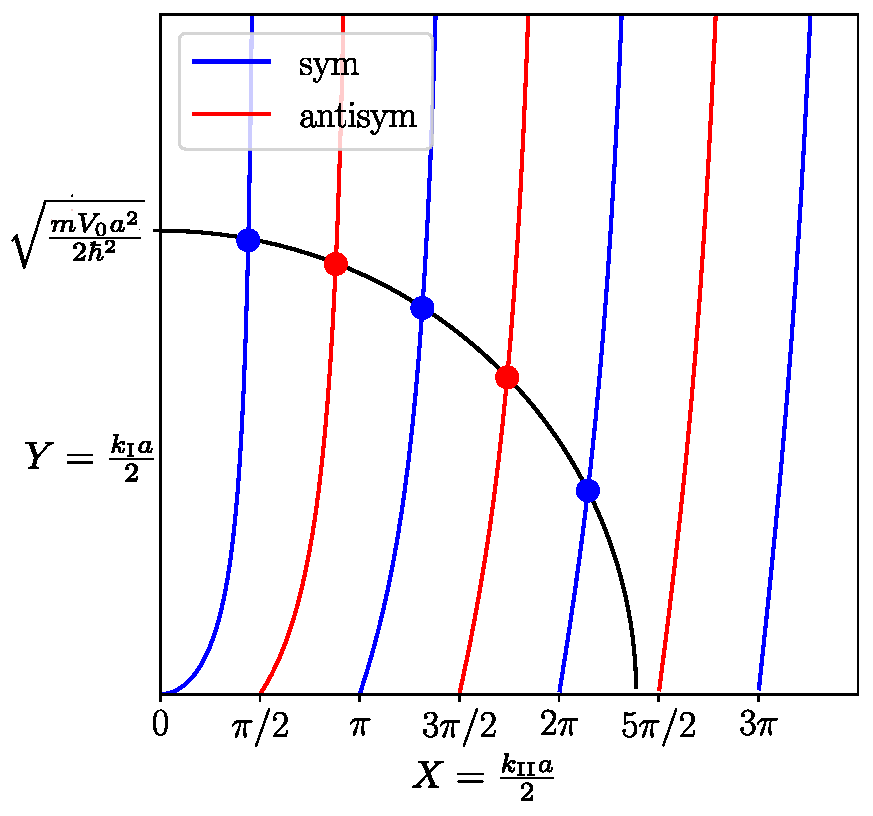
\includegraphics[width=0.6\textwidth]{Figures/modes_k_puits_fini.pdf}
% \caption{Résolution graphique pour la détermination des énergies propres des états liés symétriques (S) et antisymétriques (A) du puits de potentiel fini. On a représenté $X\to X\tan(X)$ en bleu, $X\to -X\text{cotan}(X)$ en rouge et le cercle de rayon $\sqrt{\frac{mV_0L^2}{2\hbar^2}}$ en noir. Les solutions de l'équation de Schrödinger stationnaire (modes propres) correspondent aux intersections indiquées par un cercle coloré entre les fonctions précédentes et le cercle. %La courbe a été tracée pour $\hbar=\SI{1}{ua}$, $m=\SI{1}{ua}$, $L=\SI{1}{ua}$ et $V_0=\SI{100}{ua}$.
% Dans l'exemple représenté (correspondant à une certaine valeur de $V_0$) on dénombre 3 états liés symétriques, et 2 antisymétriques.}
% \label{fig:puits_fini_2}
% \end{figure}
%
% Le système se réduit à nouveau à deux équations et deux inconnues ($A_{\rm{I}}$ et $B_{\rm{II}}$)
% \begin{equation}
% \begin{cases}
% A_\mathrm{I}\,\e^{-\frac{k_\mathrm{I}L}{2}}=-A_\mathrm{II}\sin\left(\frac{k_\mathrm{II}L}{2}\right),\\
% k_\mathrm{I}A_\mathrm{I}\,\e^{-\frac{k_\mathrm{I}L}{2}}=k_\mathrm{II}A_\mathrm{II}\cos\left(\frac{k_\mathrm{II}L}{2}\right),
% \end{cases}
% \end{equation}
% qui admet pour solution
% \begin{equation}
% .
% \end{equation}
%
%
% L'Éq.~\eqref{eqn:cercle_k1_k2} étant toujours correcte, les solutions dans le cas antisymétrique se trouvent aux intersections du cercle avec la courbe représentative de la fonction $Y=-X\mathrm{cotan}(X)$. On remarque sur la Fig.~\ref{fig:puits_fini_2} que l'état fondamental est un état symétrique, tandis que le premier état excité est antisymétrique.

\begin{remarque}
On peut utiliser le confinement d'une particule dans un puits pour préparer un ensemble de particules dans le même état quantique. Par exemple si $\sqrt{\frac{mV_0 L^2}{2\hbar^2}}<\frac{\pi}{2}$ c'est-à-dire $V_0<\frac{\hbar^2\pi^2}{2mL^2}$, il n'y a qu'un seul état lié dans le puits, qui est l'état fondamental d'énergie $E_1$. Les particules se trouvent alors toutes dans l'état fondamental.
\end{remarque}

\subsection{Expressions des modes propres}
Lorsque les conditions ci-dessus sont vérifiées, on peut exprimer les modes propres symétriques et antisymétriques à partir d'une seule constante $A_{\rm I}$, qu'on peut ensuite déterminer grâce à la normalisation de la fonction d'onde.
\begin{liste}
  \item
Les modes \imp{symétriques} s'écrivent comme
\begin{equation}
\varphi_\mathrm{S}(x)=
\begin{cases}
A_{\rm{I}}\,\e^{k_\mathrm{I}x} \text{ si } x<-\frac{a}{2},\\
A_{\rm{I}} \e^{-Y}\dfrac{\cos\left(k_\mathrm{II} x\right)}{{\cos X}} \text{ si } -\frac{a}{2}<x<\frac{a}{2}, \\
A_{\rm{I}}\,\e^{-k_\mathrm{I}x} \text{ si } x>\frac{a}{2}.
\end{cases}
\end{equation}
% \begin{remarque}
% On peut déterminer $A_{\rm{I}}$ explicitement en utilisant la normalisation de la fonction d'onde globale ($\int_{\mathbb{R}}\varphi_{\rm{S}}^2(x)\d x=1$). Le calcul se fait en séparant l'intégrale sur les différents domaines.
% \end{remarque}
\item
Les modes \imp{antisymétriques} s'écrivent comme
\begin{equation}
\varphi_\mathrm{A}(x)=\begin{cases}
A_\mathrm{I}\,\e^{k_\mathrm{I}x} \text{ si } x<-\frac{a}{2},\\
-A_{\rm{I}}\e^{-Y}\dfrac{\sin\left(k_\mathrm{II} x\right)}{{\sin X}} \text{ si } -\frac{a}{2}<x<\frac{a}{2}, \\
-A_\mathrm{I}\,\e^{-k_\mathrm{I}x} \text{ si } x>\frac{a}{2}.
\end{cases}
\end{equation}
\end{liste}

L'ensemble des modes pour l'exemple précédent est représenté en Fig.~\ref{fig:puits_fini_fonction_onde_proba_energies}.

\begin{figure}[h!]
 \centering
 
\includegraphics[width=\textwidth]{courbes_puits_fini.pdf}
 \caption{Niveaux d'énergie, et représentation de la partie spatiale de la fonction d'onde et de la densité de probabilité associée pour chaque mode. On notera l'alternance d'un mode symétrique et d'un mode antisymétrique, l'énergie non nulle du mode fondamental et surtout la probabilité de présence non nulle de la particule à l'extérieur du puits pour $\abs{x}>\frac{L}{2}$ même si les états sont ici liés ($E<V_0$), ce qui est un effet purement quantique.}
 \label{fig:puits_fini_fonction_onde_proba_energies}
 \end{figure}
 \clearpage

 \subsection{Élargissement effectif du puits par les ondes évanescentes}
On observe sur la Fig.~\ref{fig:puits_fini_fonction_onde_proba_energies} que la probabilité de présence de la particule en dehors du puits (dans les régions I et III) est non nulle! La fonction d'onde est \important{évanescente} (elle décroît exponentiellement) dans les régions I et III. La fonction d'onde pénètre dans ces régions sur une distance typique
\begin{equation}
\delta=\frac{1}{k_{\rm{I}}}=\frac{\hbar}{\sqrt{2m(V_0-E)}}
\end{equation}
On remarque tout d'abord que cet effet est purement quantique (présence de la constante $\hbar$), mais on peut le rapprocher des phénomènes ondulatoires classiques, comme l'effet de peau.
% La longueur de pénétration augmente lorsque l'énergie propre se rapproche de l'énergie nécessaire pour franchir la barrière, ce que l'on constate effectivement dans la résolution numérique en Fig.~\ref{fig:puits_fini_fonction_onde_proba_energies}.

Notons qu'une particule classique ne peut pas explorer les régions I et III avec $E<V_0$ cela impliquerait que l'énergie cinétique $E_c = E-V_0$ serait négative ! En revanche, la mécanique quantique autorise une particule à explorer cette région sur une distance de l'ordre de $\delta$. Ainsi, la fonction d'onde s'étend sur une distance totale de l'ordre de $a_{\rm eff} \simeq a+2\delta$. La largeur effective du puits fini est donc supérieure à celle du puits fini.

En conséquence, les énergies de point zéro pour le puits infini et pour le puits fini sont différentes. On voit que le \imp{mode fondamental} du puits fini vérifie $\frac{k_\mathrm{II}L}{2}<\frac{\pi}{2}$, et donc possède une énergie
\begin{equation}
  E_{1,{\rm fini}} = \frac{\hbar^2 k_{\rm{II}}^2}{2m} < \frac{\hbar^2\pi^2}{2ma^2} =   E_{1,{\rm infini}} .
\end{equation}
\begin{prop}\label{prop:}
  Dans le puits fini, l'\imp{énergie de point zéro est inférieure} à celle du puits infini.
\end{prop}
% En utilisant l'Éq.~(\ref{eqn:energie_confinement}), cela suggère que la particule dans le puits fini est confinée sur une taille caractéristique supérieure à la taille de confinement dans le cas du puits infini, qui est $L$. Cet élargissement effectif du puits est causé par l'existence d'ondes évanescentes en dehors du puits fini, qui génèrent une probabilité de présence non nulle de la particule en dehors du puits. Ainsi, la particule quantique peut sortir du puits, sur une longueur caractéristique $\delta\simeq 1/k_\mathrm{I}$, de sorte qu'elle est confinée sur une taille caractéristique $L_\mathrm{eff}=L+2\delta>L$.


\section{La barrière de potentiel et l'effet tunnel}
\subsection{Position du problème}

\begin{figure}[h!]
\centering

\includegraphics[width=0.55\textwidth]{barriere.pdf}
\caption{Représentation du potentiel $V(x)$ dans le cas de la barrière de potentiel de \guill{hauteur} $V_0$.}
\label{fig:barriere}
\end{figure}

Nous étudions pour finir le cas d'une particule libre venant de $x\to-\infty$ qui rencontre une barrière de potentiel d'épaisseur $a$ et d'amplitude $V_0>0$ Autrement dit, la particule évolue dans le potentiel schématisé Fig.~\ref{fig:barriere} tel que
\begin{equation}
V(x)=\begin{cases}
0 \text { si } x<-\frac{a}{2},\\
V_0 \text{ si } -\frac{a}{2}<x<\frac{a}{2},\\
0 \text { si } x>\frac{a}{2}.
\end{cases}
\end{equation}

En mécanique \imp{classique}, une particule de masse $m$ dans ce potentiel est d'énergie totale $E = E_c + V(x)$ constant, avec $E_c>0$ l'énergie cinétique. On peut alors distinguer plusieurs cas selon la valeur de son énergie $E$ :
\begin{liste}
\item $E<0$ : la particule ne peut pas exister dans l'espace ;
\item $0\leq E<V_0$ : la particule peut se mouvoir librement dans la région $x<-\frac{a}{2}$ mais elle ne peut pas franchir la barrière de potentiel. Elle rebondit donc sur la barrière ;
\item $E\geq V_0$ : la particule franchit la barrière de potentiel et explore ensuite la région $x>+\frac{a}{2}$.
\end{liste}
Nous allons voir que le comportement d'une particule \imp{quantique} diffère de celui d'une particule classique sous deux aspects.
\begin{liste}
  \item Pour tout $E>0$, la particule quantique a une certaine \imp{probabilité} de franchir la barrière de potentiel, mais on ne peut pas prédire si elle va effectivement la traverser ou rebondir dessus.
  \item La particule quantique \imp{peut traverser} la barrière de potentiel même si $0\leq E<V_0$ : c'est l'\imp{effet tunnel}.
\end{liste}
Dans la suite, on se propose d'étudier ce problème dans le cas où \eqbox{0\leq E<V_0.}
\subsection{États stationnaires}

\parag{Expression de la fonction d'onde}

Le rôle des régions I et III d'un côté, et II de l'autre, sont intervertis par rapport au puits de potentiel fini. L'équation de Schrödinger indépendante du temps s’écrit ici
\begin{equation}
\begin{cases}
\frac{\d^2\varphi}{\d x^2}+\frac{2mE}{\hbar^2}\varphi=0\quad\text{(régions I et III)},\\[2mm]
\frac{\d^2\varphi}{\d x^2}-\frac{2m\left(V_0-E\right)}{\hbar^2}\varphi=0\quad\text{(région II)}.
\end{cases}
\label{eqn:schro_tunnel}
\end{equation}
En posant cette fois $k_\mathrm{I}=\sqrt{\frac{2mE}{\hbar^2}}$ et $k_\mathrm{II}=\sqrt{\frac{2m\left(V_0-E\right)}{\hbar^2}}$, la partie spatiale de la fonction d'onde s'écrit :
\begin{equation}
\varphi(x)=\begin{cases}
A_\mathrm{I}\,\e^{ik_\mathrm{I}x}+B_\mathrm{I}\,\e^{-ik_\mathrm{I}x} \text{ si } x<-\frac{a}{2}, \\
A_\mathrm{II}\cosh(k_\mathrm{II}x)+B_\mathrm{II}\sinh(k_\mathrm{II}x) \text{ si } -\frac{a}{2}<x<\frac{a}{2}, \\
A_\mathrm{III}\,\e^{ik_\mathrm{I}x} \text{ si } x>\frac{a}{2},
\end{cases}
\end{equation}
où nous avons utilisé le fait que la particule venait de $-\infty$ ($B_\mathrm{III}=0$).

Le problème se résume alors à un problème ondulatoire classique. Une onde de matière incidente se propage vers un milieu, une partie est réfléchie tandis qu'une onde évanescente s'établit. En sortie du milieu, une onde propagative est transmise. On va donc par la suite définir les ondes de matière \imp{incidente, réfléchie et transmise} respectivement telles que
\begin{equation}
\begin{split}
\psi_\mathrm{i}(x,t)&=A_\mathrm{I}\,\e^{i(k_\mathrm{I}x-iE/\hbar t)},\\
\psi_\mathrm{r}(x,t)&=B_\mathrm{I}\,\e^{i(-k_\mathrm{I}x-iE/\hbar t)},\\
\psi_\mathrm{t}(x,t)&=A_\mathrm{III}\,\e^{i(k_\mathrm{I}x-iE/\hbar t)}.
\end{split}
\end{equation}

\parag{Coefficient de transmission}
Par analogie avec les ondes électromagnétiques, on peut définir des coefficients de réflexion et transmission en probabilité à travers la barrière, à partir des courants de probabilité, tels que
\begin{theorem}[Coefficients de réflexion et transmission]\label{form:}
  \begin{equation*}
  R=\frac{\left\vert B_\mathrm{I}\right\vert^2}{\left\vert A_\mathrm{I}\right\vert^2}, \hspace*{.3cm} T=\frac{\left\vert A_\mathrm{III}\right\vert^2}{\left\vert A_\mathrm{I}\right\vert^2},
\end{equation*}
  où $R+T=1$ d'après la conservation du courant de probabilité.
\end{theorem}
 La détermination explicite de ces coefficients est fastidieuse et ne figure pas au programme. On donne juste ici leurs expressions

\begin{equation}
R=\frac{\displaystyle\frac{V_0^2}{4E(V_0-E)}\sinh^2(k_\mathrm{II}L)}{\displaystyle 1+\frac{V_0^2}{4E(V_0-E)}\sinh^2(k_\mathrm{II}L)},\hspace*{0.3cm} T=\frac{1}{\displaystyle 1+\frac{V_0^2}{4E(V_0-E)}\sinh^2(k_\mathrm{II}L)}.
\end{equation}
% En particulier, on note que la relation $R+T=1$ qui traduit la (associé à la conservation de la norme de la fonction d'onde) est bien vérifiée.

\subsection{Effet tunnel}
En présence d'une barrière de potentiel de hauteur $V_0$, le coefficient de transmission $T$ d'une particule quantique de masse $m$ et d'énergie $E<V_0$ est non nul. Contrairement à la prédiction classique, il existe une probabilité non nulle que la particule traverse la barrière. Cette effet provient de l'existence d'une onde évanescente de matière qui pénètre la barrière sur une épaisseur de peau
% \begin{equation}
  \eqbox[]{
    \delta=\frac{1}{k_\mathrm{II}}=\frac{\hbar}{\sqrt{2m(V_0-E)}}.
    }
% \end{equation}

\begin{definition}[Effet tunnel]\label{def:}
  On appelle \imp{effet tunnel} l'effet quantique qui permet à une particule d'énergie $E$ de franchir une barrière de potentiel de hauteur $V_0>E$ avec une probabilité $T$ non nulle.
\end{definition}

Dans l'hypothèse d'une \important{barrière épaisse} $L\gg \delta$, un développement limité de $T$ donne
% \begin{equation}
  \eqbox[]{
    T\simeq \frac{16E(V_0-E)}{V_0^2}\,e^{-\frac{2L}{\delta}}.
    }
% \label{eqn:Ttunnel}
% \end{equation}
Le coefficient de transmission en probabilité décroît exponentiellement avec l'épaisseur $a$ de la barrière, et augmente quand $m$ diminue ou $E$ augmente. L'effet tunnel permet d'expliquer le principe de la microscopie à effet tunnel et le mécanisme de la désintégration alpha.
\end{document}
